%==============================================================================
% Sjabloon onderzoeksvoorstel bachelorproef
%==============================================================================
% Gebaseerd op LaTeX-sjabloon ‘Stylish Article’ (zie voorstel.cls)
% Auteur: Jens Buysse, Bert Van Vreckem
%
% Compileren in TeXstudio:
%
% - Zorg dat Biber de bibliografie compileert (en niet Biblatex)
%   Options > Configure > Build > Default Bibliography Tool: "txs:///biber"
% - F5 om te compileren en het resultaat te bekijken.
% - Als de bibliografie niet zichtbaar is, probeer dan F5 - F8 - F5
%   Met F8 compileer je de bibliografie apart.
%
% Als je JabRef gebruikt voor het bijhouden van de bibliografie, zorg dan
% dat je in ``biblatex''-modus opslaat: File > Switch to BibLaTeX mode.

\documentclass{voorstel}
\usepackage{tabularx}
%------------------------------------------------------------------------------
% Metadata over het voorstel
%------------------------------------------------------------------------------

%---------- Titel & auteur ----------------------------------------------------

% TODO: geef werktitel van je eigen voorstel op
\PaperTitle{Zal een progressive web app de native app vervangen?}
\PaperType{Onderzoeksvoorstel Bachelorproef 2019-2020} % Type document

% TODO: vul je eigen naam in als auteur, geef ook je emailadres mee!
\Authors{Robbie Verdurme\textsuperscript{1}} % Authors
\CoPromotor{Bart Delrue\textsuperscript{2} (Digipolis)}
\affiliation{\textbf{Contact:}
   \textsuperscript{1} \href{mailto:robbie.verdurme.y9234@student.hogent.be}{robbie.verdurme.y9234@student.hogent.be}; \textsuperscript{2} \href{mailto:bart.delrue@digipolis.be}{bart.delrue@digipolis.be};
}

%---------- Abstract ----------------------------------------------------------

\Abstract{
De native app is al even de voornaamste manier om apps te ontwikkelen. Deze heeft een groot nadeel als er zowel voor android als voor ios een applicatie ontwikkeld moet worden. Dan zijn er immers verschillende code bases die onderhoud vereisen. Daaruit is het cross-platform development ontstaan. Dit staat nog niet op punt. Gelijktijdig werkten de webdevelopers aan een oplossing voor dit probleem. Deze hebben nu een oplossing namelijk een PWA. Een PWA heeft als grote voordeel dat er maar één codebase is voor de meeste platformen. Safari ondersteunt de service worker nog niet. Om die reden worden beide oplossingen momenteel vergeleken op vlak van snelheid en benodigde ruimte. De verwachtingen van deze paper zijn dat de PWA minder ruimte vraagt op het apparaat omwille van de service worker die in de PWA verwerkt zit. Deze gaat alle data die opgevraagd wordt bijhouden (cashen), zodat deze later offline beschikbaar zijn. Dit zorgt ervoor dat de PWA een paar milliseconden trager laadt dan de traditionele native app.
%	Hier schrijf je de samenvatting van je voorstel, als een doorlopende tekst van één paragraaf. Wat hier zeker in moet vermeld worden: \textbf{Context} (Waarom is dit werk belangrijk?); \textbf{Nood} (Waarom moet dit onderzocht worden?); \textbf{Taak} (Wat ga je (ongeveer) doen?); \textbf{Object} (Wat staat in dit document geschreven?); \textbf{Resultaat} (Wat verwacht je van je onderzoek?); \textbf{Conclusie} (Wat verwacht je van van de conclusies?); \textbf{Perspectief} (Wat zegt de toekomst voor dit werk?).
%	Bij de sleutelwoorden geef je het onderzoeksdomein, samen met andere sleutelwoorden die je werk beschrijven.	
%	Vergeet ook niet je co-promotor op te geven.
}

%---------- Onderzoeksdomein en sleutelwoorden --------------------------------
% TODO: Sleutelwoorden:
%
% Het eerste sleutelwoord beschrijft het onderzoeksdomein. Je kan kiezen uit
% deze lijst:
%
% - Mobiele applicatieontwikkeling
% - Webapplicatieontwikkeling
% - Applicatieontwikkeling (andere)
% - Systeembeheer
% - Netwerkbeheer
% - Mainframe
% - E-business
% - Databanken en big data
% - Machineleertechnieken en kunstmatige intelligentie
% - Andere (specifieer)
%
% De andere sleutelwoorden zijn vrij te kiezen

\Keywords{Webapplicatieontwikkeling --- Kotlin --- Vue.js --- Progressive web app(PWA) } % Keywords
\newcommand{\keywordname}{Sleutelwoorden} % Defines the keywords heading name

%---------- Titel, inhoud -----------------------------------------------------

\begin{document}

\flushbottom % Makes all text pages the same height
\maketitle % Print the title and abstract box
\tableofcontents % Print the contents section
\thispagestyle{empty} % Removes page numbering from the first page

%------------------------------------------------------------------------------
% Hoofdtekst
%------------------------------------------------------------------------------

% De hoofdtekst van het voorstel zit in een apart bestand, zodat het makkelijk
% kan opgenomen worden in de bijlagen van de bachelorproef zelf.
\graphicspath{ {./Img/} }

%---------- Inleiding ---------------------------------------------------------

\section{Introductie} % The \section*{} command stops section numbering
\label{sec:introductie}
De native app kende de afgelopen jaren een enorme groei in aantal gebruikers en werd de voornaamste manier om apps te maken. Er was oorspronkelijk wel een groot nadeel, namelijk dat de app apart moest worden geprogrammeerd voor android en voor ios. Hierdoor waren er verschillende code bases waardoor het onderhoud van de app moeilijker werd. Dit werd later opgelost door cross-platform development. Het nadeel hiervan is dat de categorieën zich vandaag niet meer beperken tot smartphone en tablets. Daarnaast blijft de app ook kampen met onderhoudsproblemen, vanwege bepaalde features die enkel beschikbaar zijn op ios. Aldus werd er verder gezocht naar een oplossing. Die is er nu, namelijk de progressive web app (PWA). Dit is een app die je gemakkelijk kan installeren op zowel android als op ios. Hierdoor los je het probleem op van de native apps. Namelijk dat een PWA maar 1 code base heeft voor alle platformen(\cite{Why_PWA_over_NativeApp}).
% onderzoeksvragen
Deze bachlorproef beseert zich op de volgende onderzoeksvragen.
\begin{itemize}
	\item Wat zijn de voordelen van PWA vs Cross-Platform Native Apps?
	\item Welke frameworks komen hiervoor in aanmerking?
	\item Wat is de impact op de gebruikerservaring en toegankelijkheid ?
	\item Zal de PWA de native app vervangen?
	
\end{itemize}

%Intro
%Hier introduceer je werk. Je hoeft hier nog niet te technisch te gaan.

%Je beschrijft zeker:

%\begin{itemize}
%  \item de probleemstelling en context
%  \item de motivatie en relevantie voor het onderzoek
%  \item de doelstelling en onderzoeksvraag/-vragen
%Mobiele applicatieontwikkeling\end{itemize}

%---------- Stand van zaken ---------------------------------------------------

\section{Stand van zaken}
\label{sec:stand van zaken}
Er zijn reeds onderzoeken uitgevoerd die de verschillende
voor- en nadelen van een PWA en van een Cross-Platform app met elkaar vergelijken. Aldus onderzoekt men de mogelijkheid om native apps te vervangen door progressive web apps.
Deze onderzoeken staan beschreven in artikels zoals die van \cite{PWA_vs_Cross-Platform}, \cite{Tinder_PWA} en \cite{Webview_PWA}

Uit onderzoek van \cite{Tinder_PWA} blijkt dat een PWA de performantie toch wel kan verhogen in vergelijking met een native app. Dit omdat de ruimte voor de app te installeren veel kleiner is dan een native app. Daarentegen vond ik terug in artikel \cite{PWA_vs_Cross-Platform} dat er nog geen zekerheid is of een native app kan vervangen worden door een PWA.
Daarnaast stelt Marjchzak dat PWA’s nog niet supported zijn binnen het apple ecosysteem. Dit omdat safari nog geen ondersteuning biedt om een service worker te draaien op het systeem. Aangezien een service worker ervoor zorgt dat een PWA alle data cached, is deze essentieel voor het bouwen van een progressive web application. Als deze data terug moet opgehaald worden als er geen internet verbinding is, haalt hij deze van de service worker die het op zijn beurt ophaalt van de cash van het systeem. Hierdoor kan de PWA offline blijven werken eens alle data geladen is.



%Hier beschrijf je de \emph{state-of-the-art} rondom je gekozen onderzoeksdomein. Dit kan bijvoorbeeld een literatuurstudie zijn. Je mag de titel van deze sectie ook aanpassen (literatuurstudie, stand van zaken, enz.). Zijn er al gelijkaardige onderzoeken gevoerd? Wat concluderen ze? Wat is het verschil met jouw onderzoek? Wat is de relevantie met jouw onderzoek?

%Verwijs bij elke introductie van een term of bewering over het domein naar de vakliteratuur, bijvoorbeeld~\autocite{Doll1954}! Denk zeker goed na welke werken je refereert en waarom.

% Voor literatuurverwijzingen zijn er twee belangrijke commando's:
% \autocite{KEY} => (Auteur, jaartal) Gebruik dit als de naam van de auteur
%   geen onderdeel is van de zin.
% \textcite{KEY} => Auteur (jaartal)  Gebruik dit als de auteursnaam wel een
%   functie heeft in de zin (bv. ``Uit onderzoek door Doll & Hill (1954) bleek
%   ...'')

%Je mag gerust gebruik maken van subsecties in dit onderdeel.

%---------- Methodologie ------------------------------------------------------
\section{Methodologie}
\label{sec:methodologie}
Om de performantie van de verschillende apps te vergelijken zal er twee maal eenzelfde applicatie gebouwd worden. Op android wordt deze gemaakt met framework kotlin, de PWA zal gemaakt worden met behulp van het framework vue.js in combinatie met nuxt. Op deze apps zullen verschillende soorten operaties uitgevoerd kunnen worden. Elk van deze operaties zal meermaals worden uitgevoerd en ondertussen zal de snelheid getest worden. Deze verkregen resultaten zullen vervolgens met elkaar vergeleken worden om te bepalen welke applicatie het meest performant is. Naast het onderzoek naar de performantie zal er ook onderzoek worden gedaan naar hoeveel ruimte deze app inneemt op een apparaat. Ook deze resultaten zullen worden vergeleken.

%Hier beschrijf je hoe je van plan bent het onderzoek te voeren. Welke onderzoekstechniek ga je toepassen om elk van je onderzoeksvragen te beantwoorden? Gebruik je hiervoor experimenten, vragenlijsten, simulaties? Je beschrijft ook al welke tools je denkt hiervoor te gebruiken of te ontwikkelen.

%---------- Verwachte resultaten ----------------------------------------------
\section{Verwachte resultaten}
\label{sec:verwachte_resultaten}
Om de resultaten voor te stellen wordt er gebruik gemaakt van een boxplot, zoals te zien is op figuur 1. Er zal er ook nog een tabel komen die de boxplot weergeeft. De getallen die hierin terug te vinden zijn: het gemiddelde, het maximum, het minimum, eerste kwadrant en derde kwadrant. Hierdoor krijgen we een goed overzicht om de resultaten te vergelijken tussen de PWA en native app.

\begin{figure}[!h]
	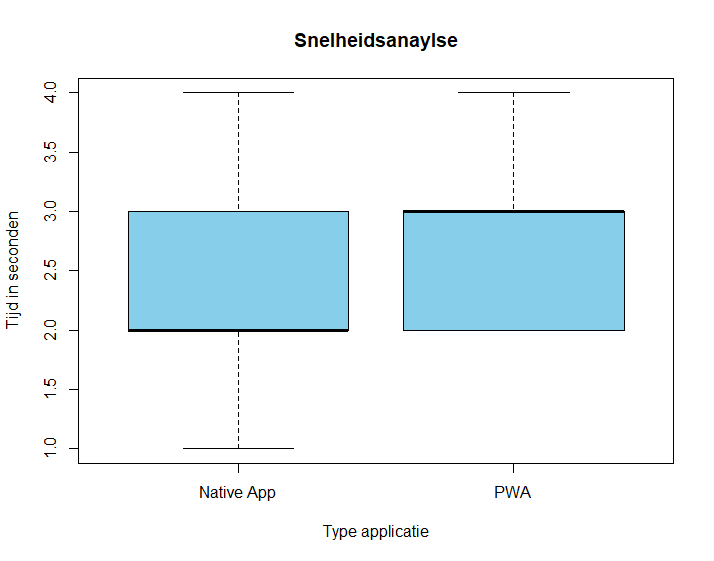
\includegraphics[width=200px]{Rplot_Boxplot_Snelheidsanalyse.png}\centering
	\caption{Voorbeeld van boxplot die de snelheid vergelijkt}
\end{figure}

\begin{figure}[!h]
	\begin{tabularx}{\textwidth /2 }{|X|X|X|X|X|X|}
		\hline
		 & min. & 1ste kwadrant & Gem. & 3de kwadrant & max. \\
		\hline
		PWA & 2 & 2 & 2.714 & 3 & 4 \\
		\hline
		native app & 1 & 1 & 2.429 & 3 & 4 \\
		\hline
	\end{tabularx}
	\caption{Voorbeeld van een tabel die de snelheid vergelijkt}
\end{figure}


Voor de resultaten van de benodigde ruimte weer te geven zal gebruik gemaakt worden van een historiek, zoals te zien is op figuur 3. Er zal zoals bij de vergelijking van de tijd ook een tabel zijn met alle info die de historiek weergeeft.

\begin{figure}[!h]
	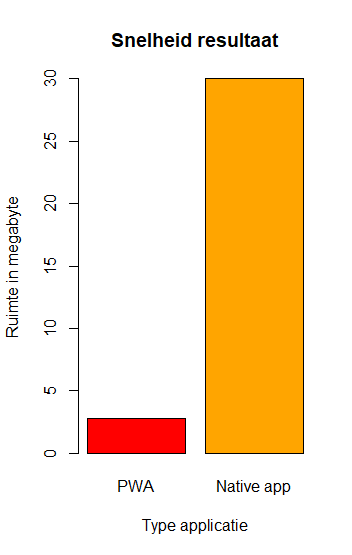
\includegraphics[width=120px]{Rplot_Ruimte_PWAvsNativeApp.png}\centering
	\caption{Voorbeeld van historgram die de benodigde ruimte vergelijkt}
\end{figure}


% tabel benodigde ruimte
\begin{figure}[!h]
\begin{tabular}{ |p{10em}|c|c| }
	\hline
	Type applicatie & Benodigde ruimte \\
	\hline
	progressive web app & 2.8 MB \\
	\hline
	native app & 30 \\
	\hline
\end{tabular}
\caption{Voorbeel van tabel die de benodigde ruimte vergelijkt}
\end{figure}


%Hier beschrijf je welke resultaten je verwacht. Als je metingen en simulaties uitvoert, kan je hier al mock-ups maken van de grafieken samen met de verwachte conclusies. Benoem zeker al je assen en de stukken van de grafiek die je gaat gebruiken. Dit zorgt ervoor dat je concreet weet hoe je je data gaat moeten structureren.

%---------- Verwachte conclusies ----------------------------------------------
\section{Verwachte conclusies}
\label{sec:verwachte_conclusies}
Er wordt verwacht dat de snelheid niet significant verschillend zal zijn tussen de PWA en de native app. De native app haalt enkel de content op waardoor deze net iets sneller zal zijn. De PWA moet alle data ophalen samen met de layout , dit is de data moet weergegeven worden. Hierdoor zal de PWA een x tal milliseconden trager zijn dan de native applicatie

Verder wordt er verwacht dat de benodigde ruimte op een apparaat significant minder zal zijn dan de native app. Dit komt doordat de native app op het apparaat zelf geïnstalleerd is. Hierdoor staat er een standaard layout geïnstalleerd op het apparaat, wat redelijk veel ruimte inneemt. De PWA haalt zowel zijn inhoud als zijn layout van een server. Hierdoor kan een PWA de benodigde ruimte op het apparaat beperken. 

%Hier beschrijf je wat je verwacht uit je onderzoek, met de motivatie waarom. Het is \textbf{niet} erg indien uit je onderzoek andere resultaten en conclusies vloeien dan dat je hier beschrijft: het is dan juist interessant om te onderzoeken waarom jouw hypothesen niet overeenkomen met de resultaten.



%------------------------------------------------------------------------------
% Referentielijst
%------------------------------------------------------------------------------
% TODO: de gerefereerde werken moeten in BibTeX-bestand ``voorstel.bib''
% voorkomen. Gebruik JabRef om je bibliografie bij te houden en vergeet niet
% om compatibiliteit met Biber/BibLaTeX aan te zetten (File > Switch to
% BibLaTeX mode)

\phantomsection
\printbibliography[heading=bibintoc]

\end{document}
